\newpage
\section{Text summarisation with SciBERT} \label{section:complex-case}

The ScoutinScience Dashboard contains a full-page evaluation view for academic publications. On this, the known metadata, historical trends about the paper's topics, social media mentions, a PDF viewer showing the document, and other augmentation tools are displayed. One of these is the \textit{Highlights} section, which aims to summarise the paper from a technology-transfer perspective.

The current approach uses a simple heuristic based on a set of phrases selected by business developers and extended with the help of a word2vec model \cite{mikolov2013efficient}. The user feedback deemed this implementation slightly helpful but inadequate for providing an accurate overview. Thus, this is the baseline I attempt to improve on in this section.

\begin{displayquote}
Compared with Section \ref{section:simple-case}, this time around, the toolset of \textit{GreatAI} is available at our disposal. Hopefully, this will streamline the development and --- especially --- the deployment. Given its arguably higher complexity, the experiment falls closer to industrial use cases and hence, can give more accurate feedback on how to further improve the API.
\end{displayquote}

\subsection{Background}

Automatic text summarisation (ATS) is also one of the earliest established tasks of text analysis and boasts numerous promising results \cite{el2021automatic}. Text summarisation is usually divided into extractive and abstractive approaches. Even though the latter can lead to more fluent summaries, it is also prone to hallucinate content that is unfaithful to the input \cite{maynez2020faithfulness}. For this reason, extractive techniques are preferred in this case.

Our problem requires generating a special type of summary: it must only concern a single aspect (tech-transfer) of the document. Aspect-based text summarisation has also seen some progress over the last decades \cite{berkovsky2008aspect,hayashi2021wikiasp}, but these methods require concretely defined topics. Unfortunately, \textit{tech-transfer potential} is anything but a clear topic definition.

Numerous discussions and interviews with business developers over the last two years made it clear that there is no universally agreed-on definition of it. At least all of them agree that they know it when they see it. Additionally, most of them agree that they can confidently make a decision on the granularity of sentences. This gives rise to an obvious idea: show the experts something they can annotate. Because experts' time is valuable, and relevant sentences are few and far between, extra care needs to be taken to improve the ratio of positive examples in the dataset. The research of Iwatsuki Kenichi on formulaic expressions (FEs) \cite{iwatsuki2020evaluation,iwatsuki2021extraction,iwatsuki2021communicative,iwatsuki2022extraction} provides a promising direction to do so. 

A formulaic expression is a phrase with zero or more ``slots'' which, when filled appropriately, leads to expressing a certain intent. In the context of scientific text, an example\footnote{Taken from the ground truth data available at \href{https://github.com/Alab-NII/FECFevalDataset/blob/master/human_evaluation/background.tsv}{github.com/Alab-NII/FECFevalDataset}.} could be: \texttt{it was not until * that}. The asterisk can be substituted with multiple terms, and the intention of this expression is (likely) to describe the \textit{History of the related topics}. Iwatsuki et al. identified a set of 39 intentions, compiled a manually labelled dataset \cite{iwatsuki2020evaluation}, and developed multiple approaches for automatically extracting and classifying formulaic expressions in large corpora \cite{iwatsuki2021communicative,iwatsuki2022extraction}.

\subsection{Methods}

In order to compile a new dataset, experts are asked to judge sentences that passed an \textit{intention check}. This pooling approach is commonly used in information retrieval \cite{schutze2008introduction}. The filtering is expected to sieve out sentences that are probably not relevant from a technology-transfer perspective using Iwatsuki's formulaic expression intention classes. Subsequently, relevance judgements --- in the form of \textit{interesting} or \textit{not interesting} labels --- are gathered for the remaining sentences. This method turns the extractive summarisation into a binary classification task for which a SciBERT model \cite{beltagy2019scibert} can be fine-tuned. Ultimately, the summaries are derived from sentences selected by the classifier trained on the experts' annotations.

We have to note two possible shortcomings of this setup: firstly, the FE intentions are assumed to be strongly correlated with the sought-after aspect. This may or may not be true. Secondly, only the individual relevance of the sentences is considered instead of the overall relevance (utility) of the summary. Nonetheless, it is expected that stemming from the length of the documents and the sparseness of the selected sentences, that any combination of them is likely to have low redundancy.

\subsection{Results}

For the first iteration, 1500 sentences were selected for two experts to annotate in a binary fashion according to strict guidelines. An example is shown in Figure \ref{fig:annotator}. Afterwards, for measuring the interrater agreement, Cohen's kappa \cite{cohen1960coefficient} is calculated as shown in Equation \ref{equation:kappa}, which turns out to be \textbf{0.4310} for the two annotators. This happens to be just above the lower end of \textit{moderate agreement}. However, we have to note that the original quality ranges are often criticised for being too relaxed \cite{mchugh2012interrater}. Regardless, in the case of summarisation, Verberne et al. \cite{verberne2018creating} argue that reasonable end-quality can be reached even when the interrater agreement is relatively low. The ground truth is determined by taking the logical disjunction of the annotations.

\begin{figure}
    \centering
    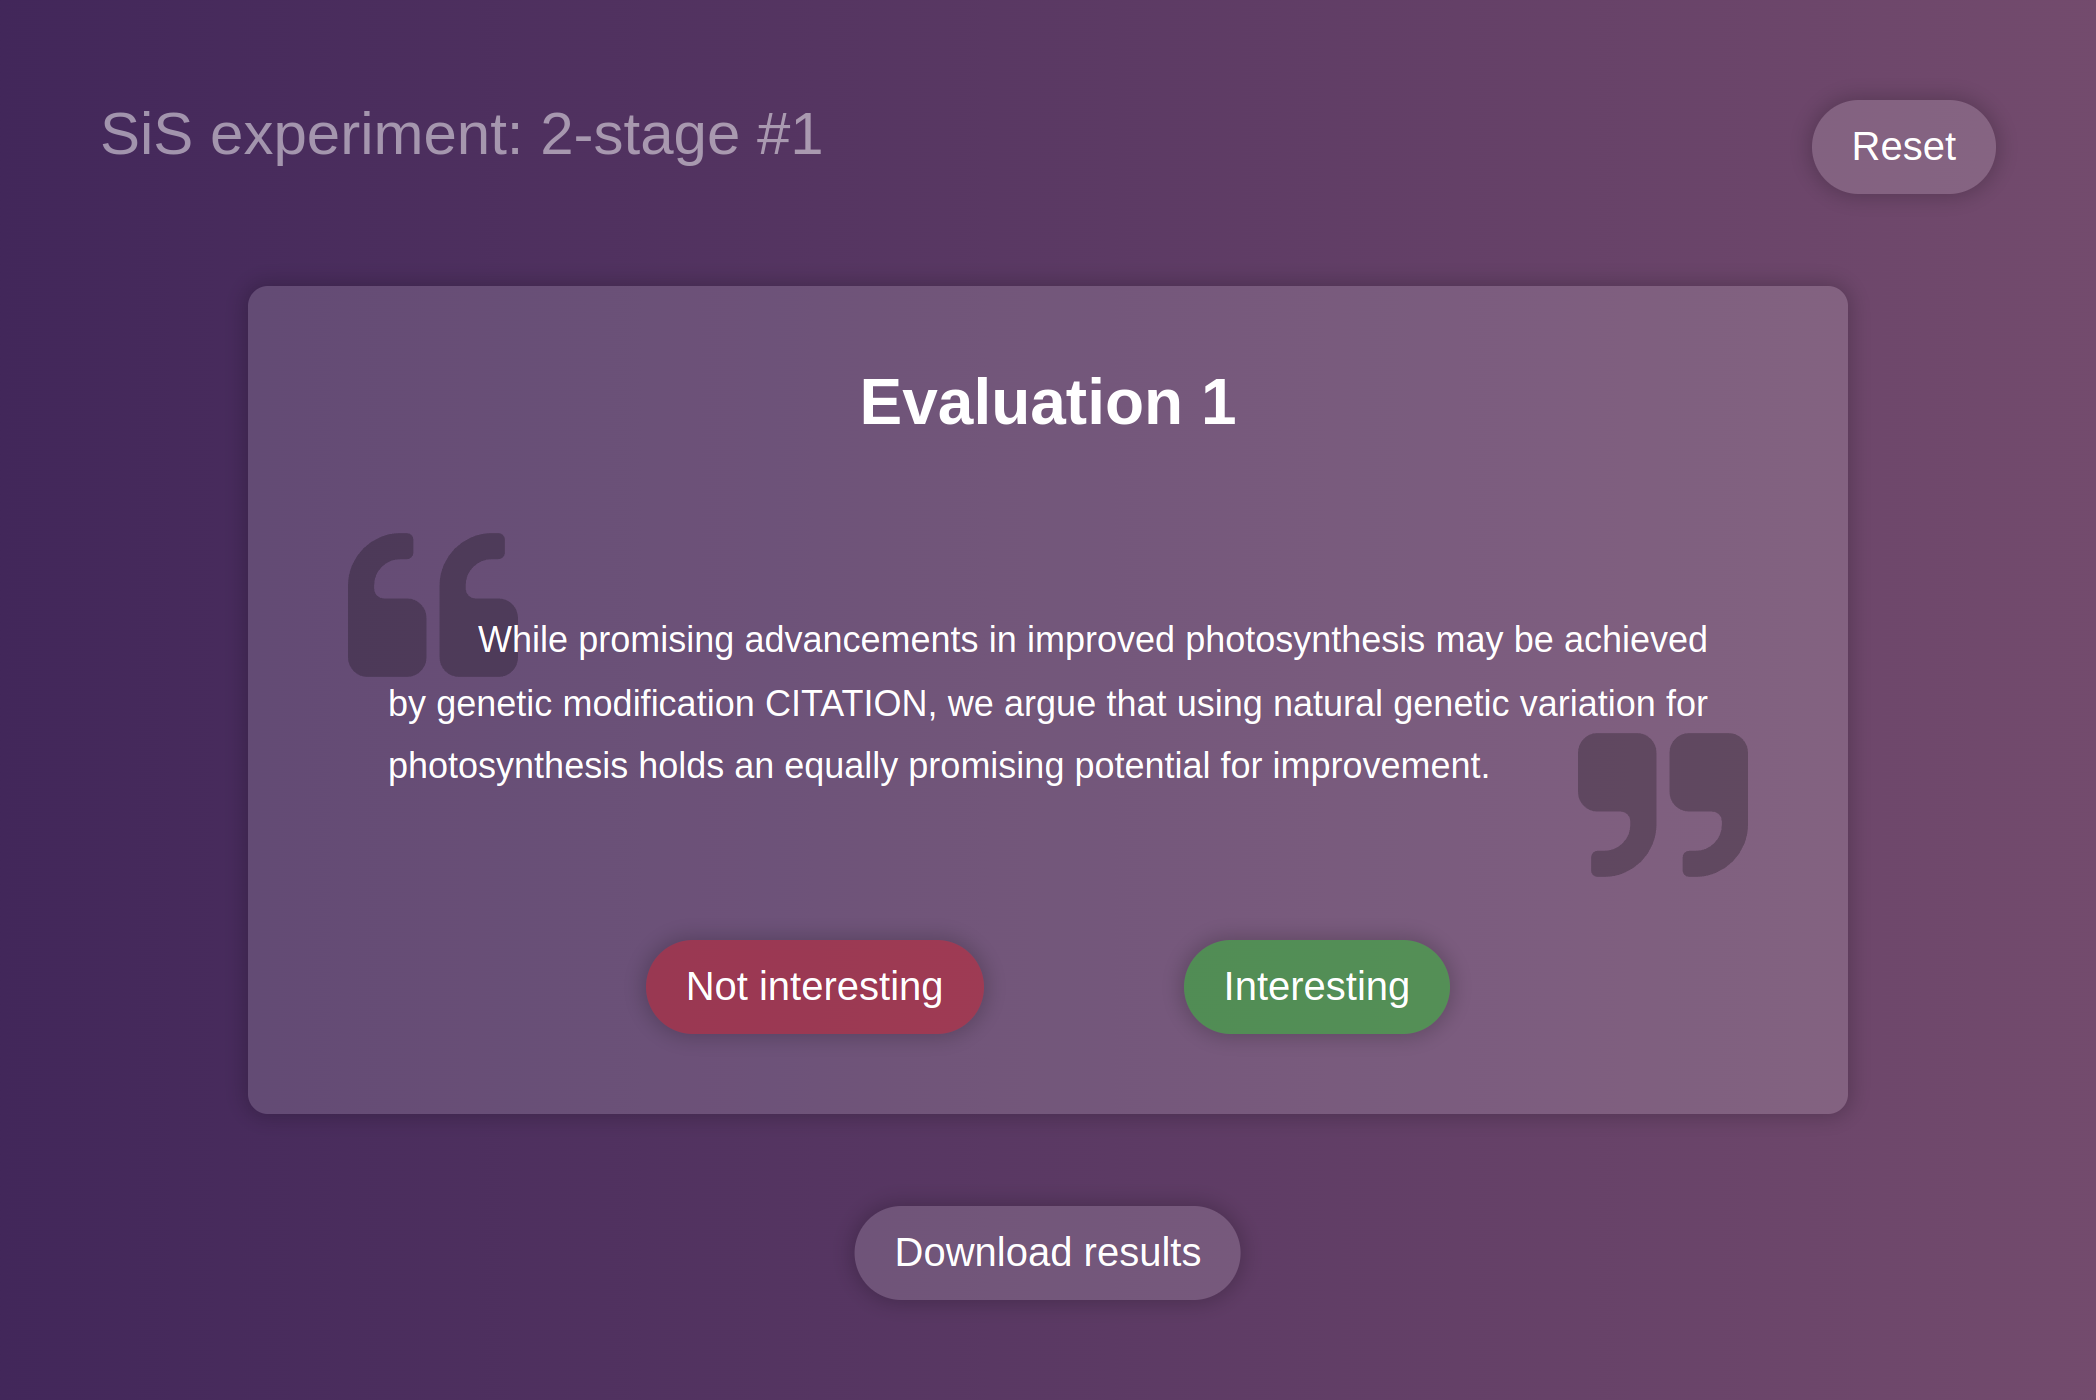
\includegraphics[width=0.75\linewidth]{figures/annotator.png}
    \captionsetup{width=.9\linewidth}
    \caption{The Annotator UI shows a single sentence and the two possible labels that can be assigned based on its relevance to technology transfer.}
    \label{fig:annotator}
\end{figure}

\begin{equation} \label{equation:kappa}
\kappa_{agreement} \equiv \frac{p_{observed} - p_{expected}}{1 - p_{expected}} = 1 - \frac{1 - p_{observed}}{1 - p_{expected}} 
\end{equation}

The next step is fine-tuning SciBERT with the help of Hugging Face \texttt{transformers} \cite{wolf2019huggingface}. The data are divided into training and test splits with a ratio of 4:1. A validation split, used for early stopping, is also derived from the train split. The objective function is the F1-score of the positive class, and the early stopping patience is five epochs. The learning rate is $5 \times 10^{-5}$ and AdamW \cite{loshchilov2017decoupled} is used for optimisation with a weight decay of 0.05. The code can be found in the documentation\footnote{\href{https://great-ai.scoutinscience.com/examples/scibert/train/}{great-ai.scoutinscience.com/examples/scibert/train}}, it is surprisingly slightly shorter than the code of Section \ref{section:simple-case}.

\begin{displayquote}
\textbf{Reproducibility} Reproducible experiments are generally preferred. It is easy to forget to set some seed values and, for example, end up with different data points in the test-train splits during training and validation in a Continuous Integration (CI) pipeline. For facilitating reproducibility, it would be useful to reset the seeds of each imported library's random number generators (RNGs) when \textit{GreatAI} is configured. Thus, a feature has been added to detect and reset RNGs of installed and imported libraries. This certainly will not solve the reproducibility crisis \cite{hutson2018artificial} on its own; however, in some cases, it can result in one fewer step to miss.
\end{displayquote}

\begin{displayquote}
\textbf{Utility of LargeFiles} For the purposes of the documentation, the fine-tuning was conducted in the Google Colab online environment, which is excellent for providing anyone with GPU time for free. However, notebook environments are ephemeral, resulting in the need to manually upload and download all relevant data whenever a new virtual machine (VM) instance is granted. The \texttt{LargeFile} implementation alleviated this problem by automatically handling the uploads and downloads. Of course, first, backwards compatibility had to be solved for Python 3.7, the only available environment in Colab.
\end{displayquote}

The best validation results were achieved after eight epochs which is slightly more than expected but is presumably due to the weight decay. The confusion matrix on the test split can be seen in Figure \ref{fig:scibert-confusion}: regardless of the task's subjective definition, SciBERT achieves good quality indicated by an F1-score of \textbf{0.89}.

\begin{figure}
    \centering
    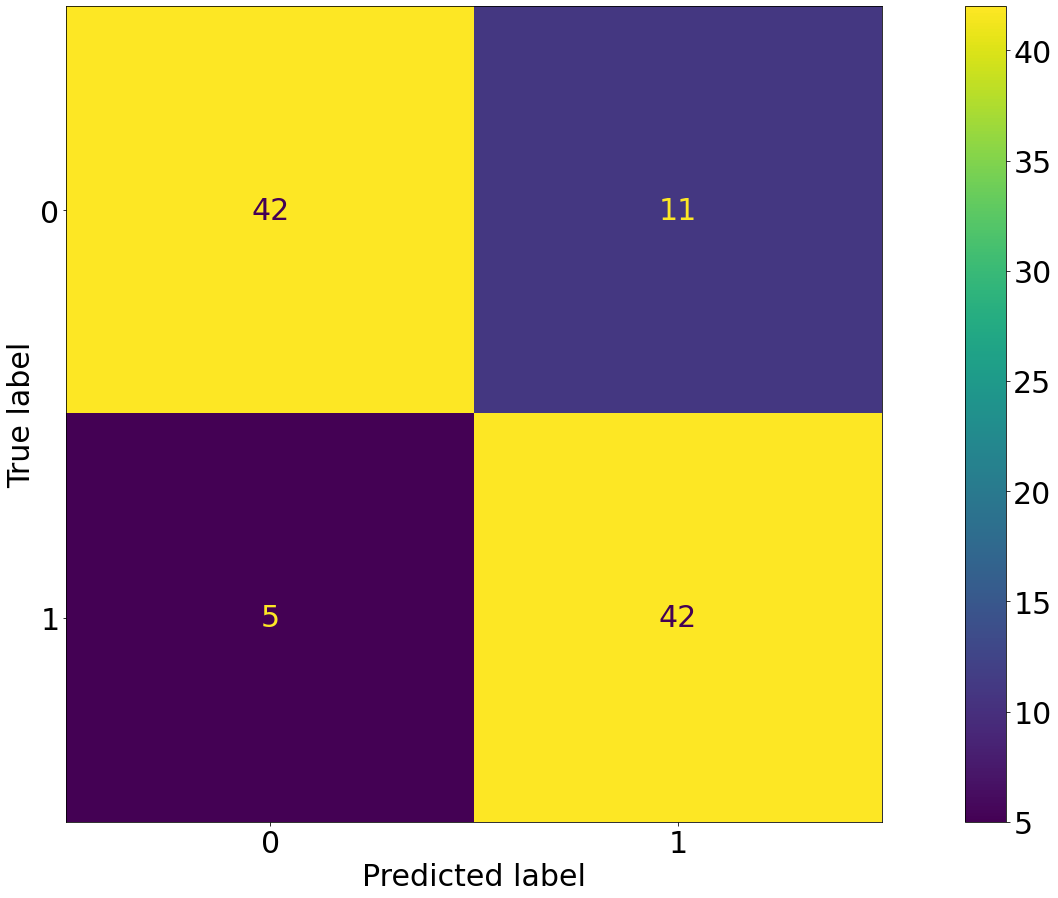
\includegraphics[width=0.4\linewidth]{figures/scibert-confusion.png}
    \captionsetup{width=.9\linewidth}
    \caption{Confusion matrix of the fine-tuned SciBERT model on the \textit{summary candidate sentences} dataset. The values are globally normalised and represent percentages.}
    \label{fig:scibert-confusion}
\end{figure}

Let us check how well the selected sentences correspond with the tech-transfer potential. Users and in-house experts can rate publications (from a tech-transfer perspective) by assigning them to one of four categories: \texttt{A}, \texttt{B}, \texttt{C}, and \texttt{D} with \texttt{A} being the most and \texttt{D} the least promising. This feedback is stored and used for analytic and training purposes. Since both the feedback grade and the ``highlights'' are supposed to reflect the same aspect of papers, therefore, we can reasonably expect some correlation between them.

Figure \ref{fig:histograms} shows the ratio of summary candidate sentences as predicted by the fine-tuned model in 4 categories (grades) of papers. This dataset does not overlap with the training data; hence, the results come solely from the model's ability to generalise. It is interesting to see that the Spearman's rank correlation coefficient \cite{spearman1961proof} between the normalised ``highlights'' counts and the ratings of papers is \textbf{0.4784} and is statistically significant ($P = 5.4 \times 10^{-74}$). This proves the presence of a monotonic association. For context, the correlation between the grades and the number of sentences chosen by the baseline approach is 0.06597 ($P = 0.03$). We can conclude that the classifier's output is indicative of publications' tech-transfer potential. 

\begin{figure}
    \centering
    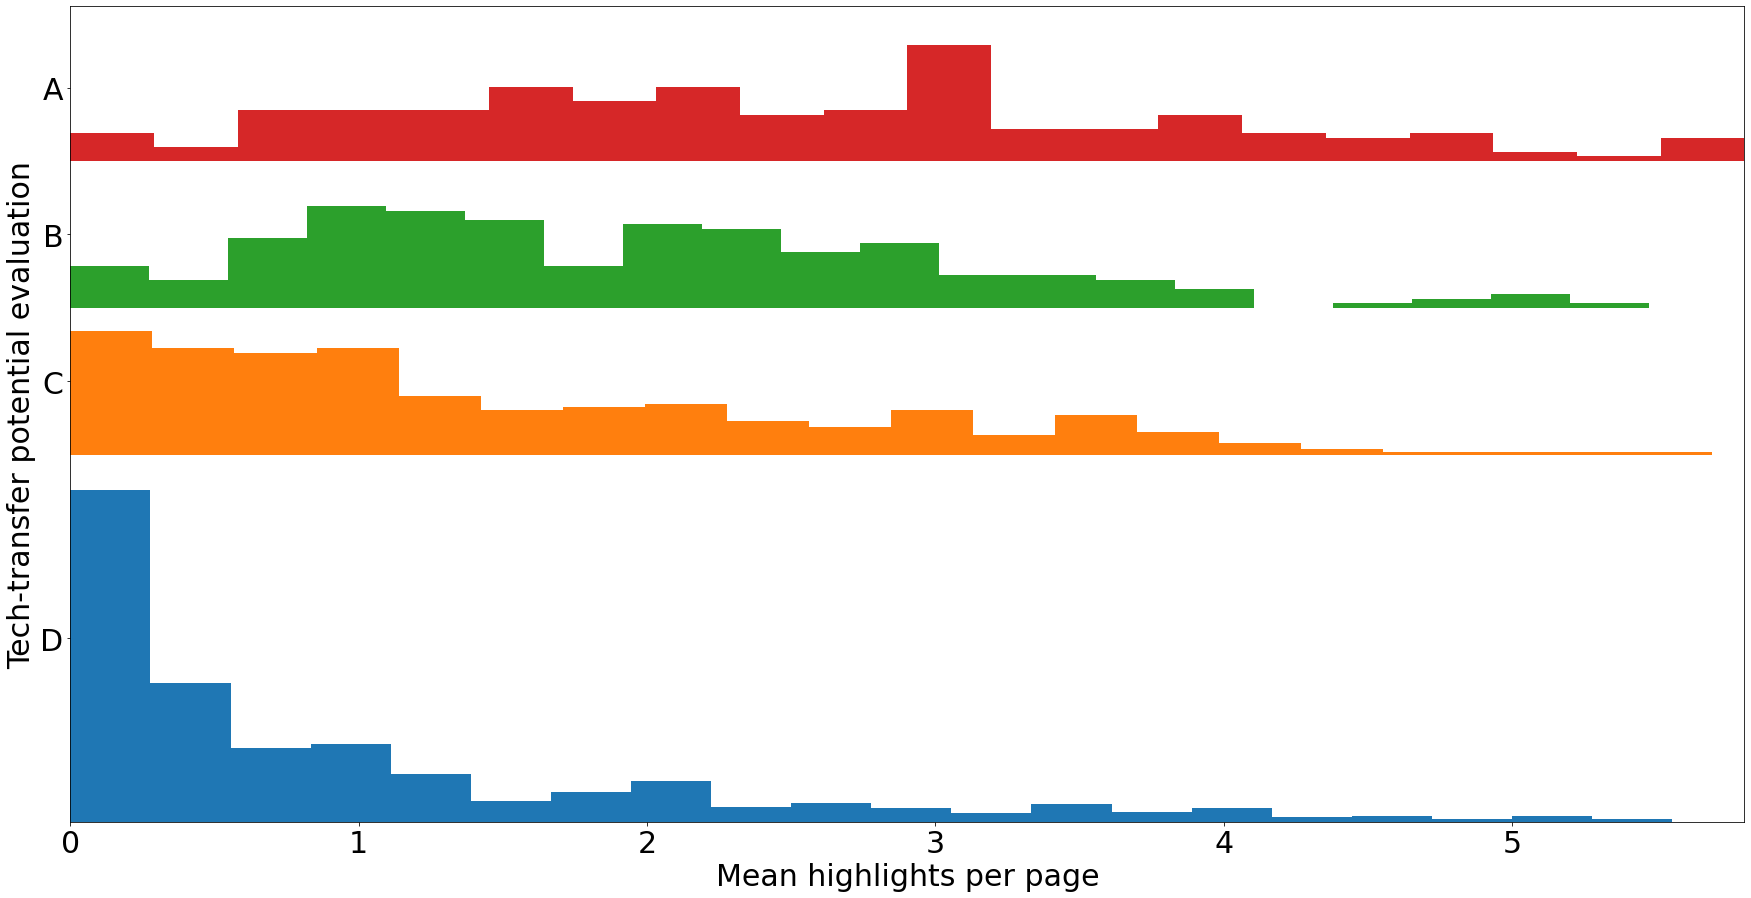
\includegraphics[width=0.85\linewidth]{figures/highlights-histograms.png}
    \captionsetup{width=.9\linewidth}
    \caption{Distribution of mean predicted summary candidate sentence counts in 4 categories. Category \texttt{A} corresponds to the most, while \texttt{D} to the least interesting papers based on mean user feedback. The sample size is 1406 (\texttt{D}=715, \texttt{C}=309, \texttt{B}=198, \texttt{A}=184). The histograms are on the same scale.}
    \label{fig:histograms}
\end{figure}

\subsection{Deployment}

To implement the summarisation, at most, the top 7 selected sentences are chosen as ranked by their log probabilities. They are subsequently reordered according to their position in the text. As a quasi-explanation, the tokens' attention scores are visualised and overlaid on the highlighted sentences. The \textit{i}-th token's visualised attention comes from summing up the attention weights of each of the last layer's heads between the \texttt{[CLS]} and the \textit{i}-th token. To improve the end-user experience, a high-pass filter and a stop-word list are applied to the scores to avoid highlighting the syntax-related tokens (punctuation, determiners). The service --- after being integrated into the dashboard --- can be seen in Figure \ref{fig:dashboard-highlights}.

\begin{displayquote}
\textbf{Design inspiration} In order to get insights into their inner workings, Hugging Face models can be given \texttt{output\_attentions=True} in their constructor, which results in a new property becoming accessible on the results for querying the attentions. The only issue with it is that it is a 5-dimensional matrix which makes exploring and understanding it non-obvious. In short, it has very low \textit{Discoveribility}. For example, the attention weights for the UI are calculated with this expression:
\begin{minted}[
baselinestretch=1,
]{python}
np.sum(result.attentions[-1].numpy()[0], axis=0)[0][1:-1]
\end{minted}
Even though the operation is conceptually simple, because of the opaque data structure, this is anything but obvious to comprehend. Therefore, it is clear that this needs to be avoided in my library design; it has to have an explicit and discoverable API that can be achieved using type hints, descriptive property names, and docstrings.
\end{displayquote}

\begin{figure}
    \centering
    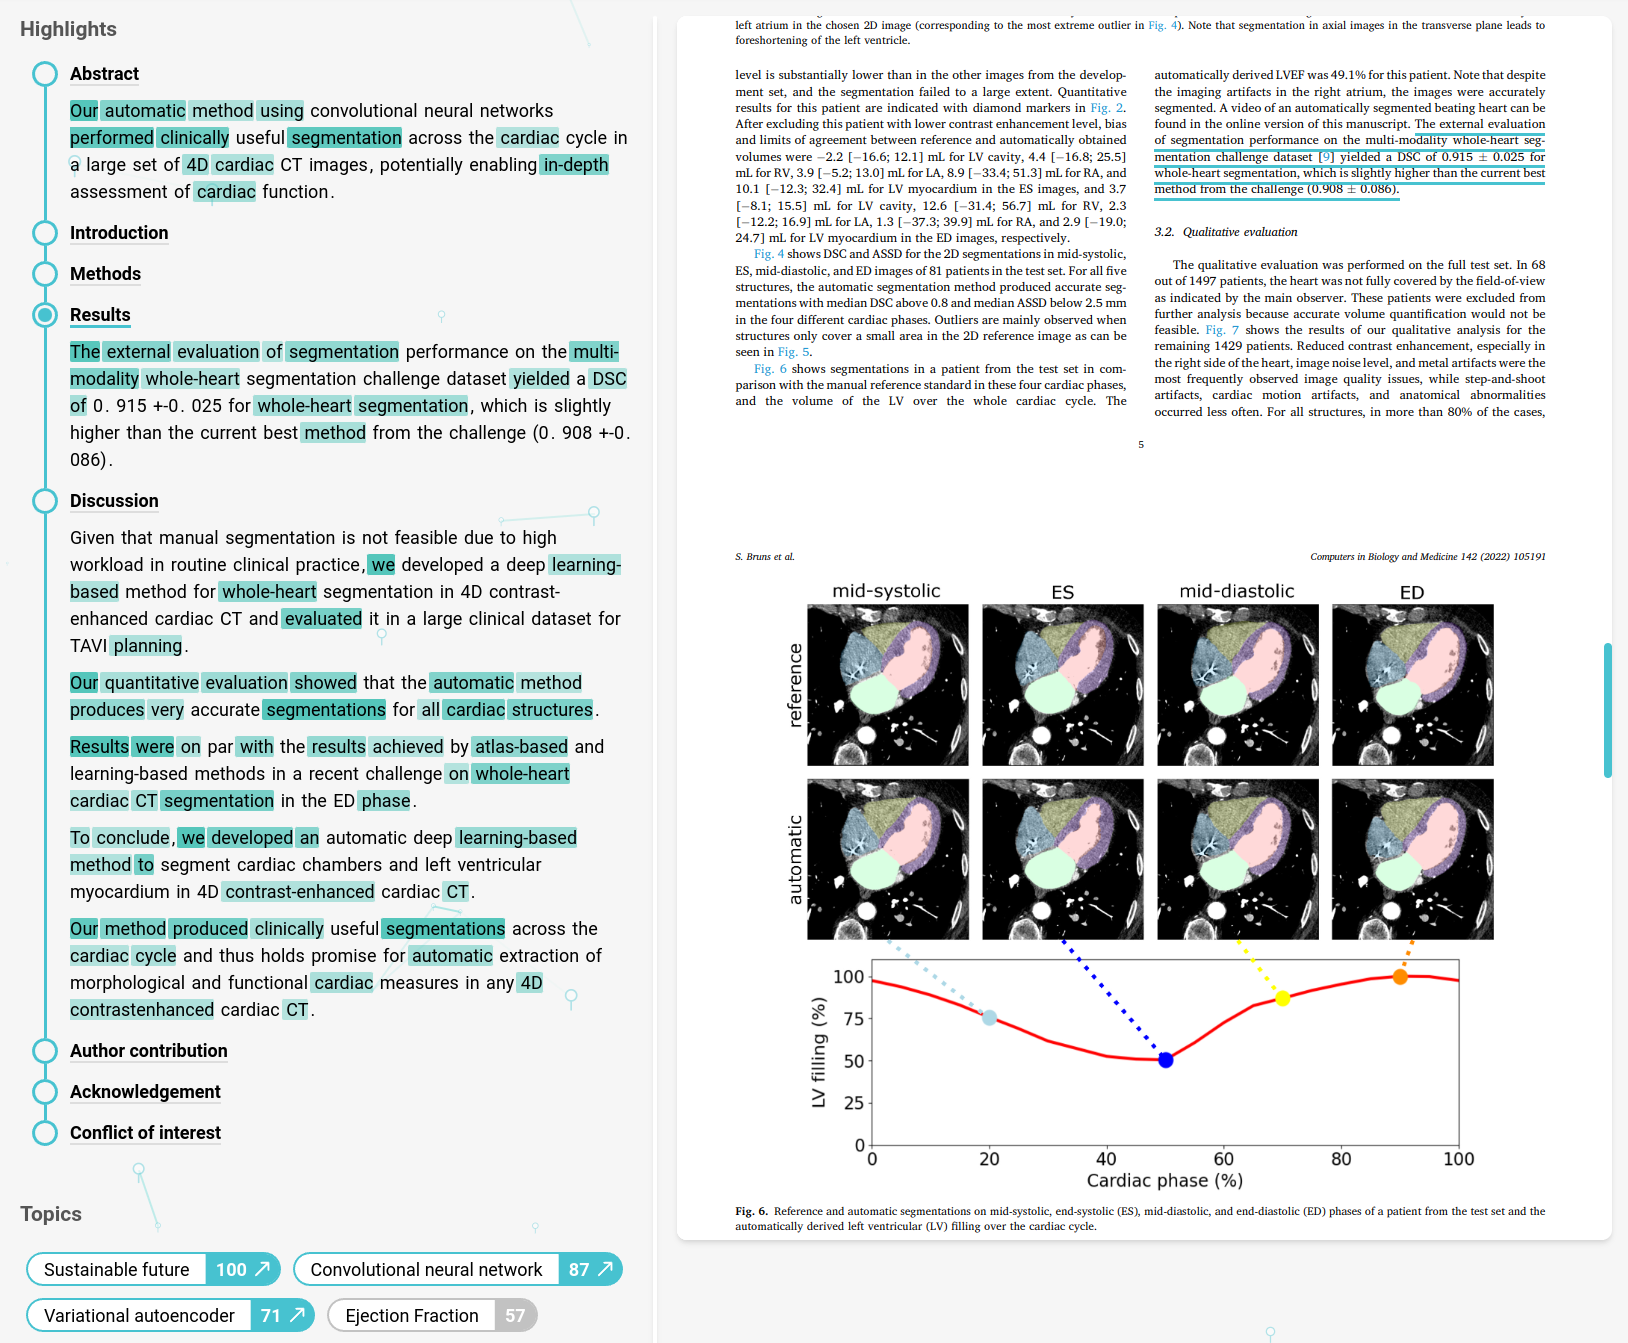
\includegraphics[width=1\linewidth]{figures/dashboard-highlights.png}
    \captionsetup{width=.9\linewidth}
    \caption{The tech-transfer summary of an academic publication (\cite{bruns2022deep}). The titles and sentences can be clicked to navigate the paper on the right. Meanwhile, some explanation is provided by the highlighted words, the opacity of which corresponds to their attention weights.}
    \label{fig:dashboard-highlights}
\end{figure}

\section{Improving GreatAI}

After having solved two problems by implementing two standalone services and integrating them into an existing ecosystem while relying on \textit{GreatAI} as a primary tool, a wide variety of insights have been gained. In the next couple of subsections, the extra features and design decisions that were motivated by the \textit{Highlights (summarisation) service} are presented. After which, the final surface of the API is described and evaluated by its relation to the SE4ML \cite{serban2020adoption,serban2021practices} and AI engineering \cite{john2020architecting,john2020ai} best practices.

\subsection{Caching}

Sustainability is an increasingly crucial concern of ethical AI \cite{van2021sustainable}. Without discussing the pros and cons of the green computing movement \cite{10.1145/1400181.1400186}, we can still agree that computing time should not be wasted. To this end, caching the results of expensive operations has to be considered in any AI deployment. In this case, the \textit{Highlights service} is often called multiple times from different other services with the same parameters. With each operation taking up to a couple of seconds, implementing caching can lead to vastly faster response times and an overall more socially conscious deployment.

\subsection{Revisiting \texttt{parallel\_map}}

Even though most inference functions are CPU-bound, it turns out that sometimes they involve IO, especially when relying on the results of other remote models. This means a significant performance improvement can be achieved by implementing some inference functions asynchronously \cite{tilkov2010node}. Thus, \textit{GreatAI} also has to support decorating both regular (synchronous) and asynchronous functions. One notable consequence is that the batch processing feature must also be compatible with \texttt{async} inference functions. Batch processing is still a helpful feature since it is likely that async inference functions are both IO (remote calls) and CPU (local evaluation) constrained at the same time. Thus, they can benefit from multi-core parallelisation. 

However, the standard library's \texttt{multiprocessing}, the third party \texttt{multiprocess} \cite{mckerns2012building}, and, another popular library, \texttt{joblib}\footnote{\href{https://joblib.readthedocs.io/en/latest/}{joblib.readthedocs.io/en/latest}} all lack the support for efficiently parallelising async functions. For this reason, \texttt{parallel\_map} is reimplemented to create an event-loop in each worker process to keep the efficiency of non-blocking IO while also providing parallelisation for the CPU-bound sections of code.

\subsection{Programmatic integration}

Apart from supporting \texttt{async} calls, a couple more steps can be taken to help integrate any service with a \textit{GreatAI} deployment. This is implemented by the \texttt{call\_remote\_great\_ai} function which hides the networking required to call a \textit{GreatAI} instance's REST API. It takes care of validation, automatic retries, serialisation, and deserialisation. It comes with the added benefit of encouraging decoupled services because the friction of integrating them is no longer noticeable, which is beneficial for human collaboration \cite{hasselbring2002component}.

Additionally, a REST API is generated with its accompanying OpenAPI schema\footnote{\href{https://swagger.io/specification}{swagger.io/specification}} and served with a \href{https://swagger.io/}{Swagger} template. It also contains metadata about the function, for instance, its docstring, version, and version of its registered models concatenated in order to be SemVer\footnote{\href{https://semver.org/}{semver.org}} compatible. These can be seen in Figure \ref{fig:greatai-api}. This, combined with a \texttt{/version} HTTP endpoint for programmatic access and validation of the service's metadata, proved to be valuable features when integrating the \textit{Highlights service} into ScoutinScience's service-based architecture.

\begin{figure}
    \centering
    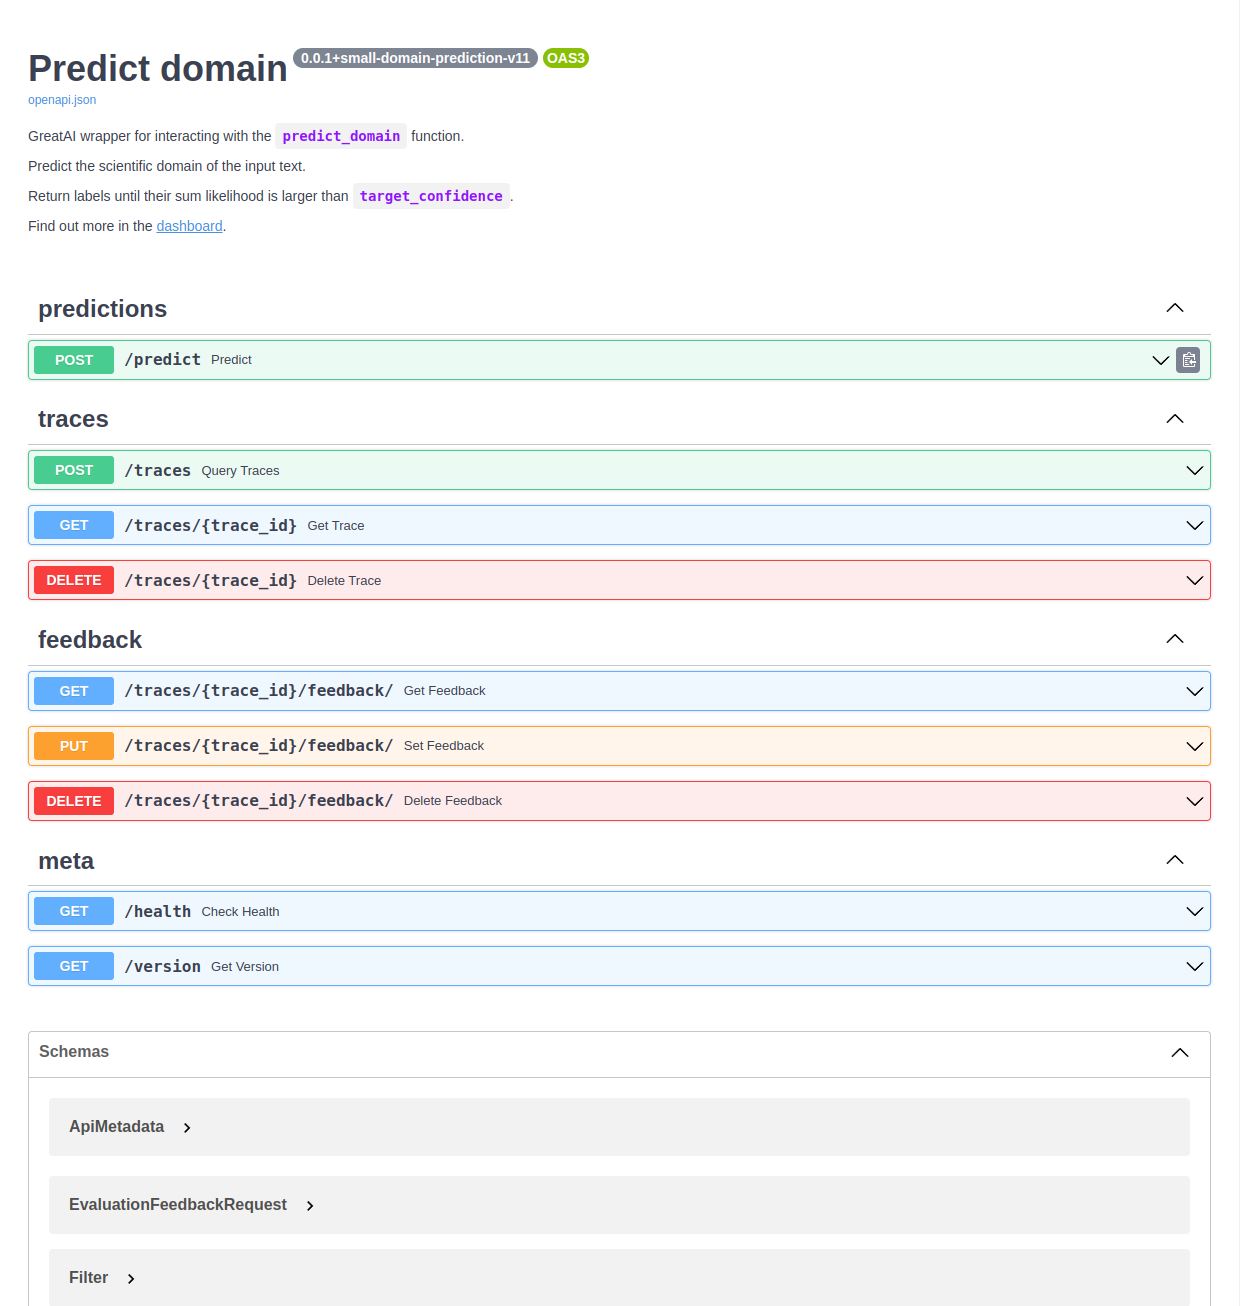
\includegraphics[width=0.85\linewidth]{figures/greatai-api.png}
    \captionsetup{width=.9\linewidth}
    \caption{Documentation of the automatically scaffolded REST API of a \textit{GreatAI} service. Notice, how its version string includes its registered models in a SemVer compliant way: \texttt{0.0.1+small-domain-prediction-v11}.}
    \label{fig:greatai-api}
\end{figure}

\subsection{Human integration}

Even though the REST API of \textit{GreatAI} services exposes all necessary features\footnote{Such as providing feedback per prediction, complexly filtering and sorting traces, create-read-update-delete (CRUD) operations for the feedbacks and traces, accessing live monitoring info (current configuration, versions, cache statistics), etc.} which are great for programmatic access, these are not ideal for direct human consumption. To ease the introduction of \textit{GreatAI} services, a rudimentary dashboard is --- optionally --- generated next to the REST API. The dashboard's main features can be observed in Figures \ref{fig:greatai-header}, \ref{fig:greatai-table}, and \ref{fig:greatai-parallel}. The diagrams and filterable/sortable table are interconnected and are automatically updated; the reactive behaviour is provided by the Dash framework \cite{shammamah_hossain-proc-scipy-2019}.

\begin{figure}
    \centering
    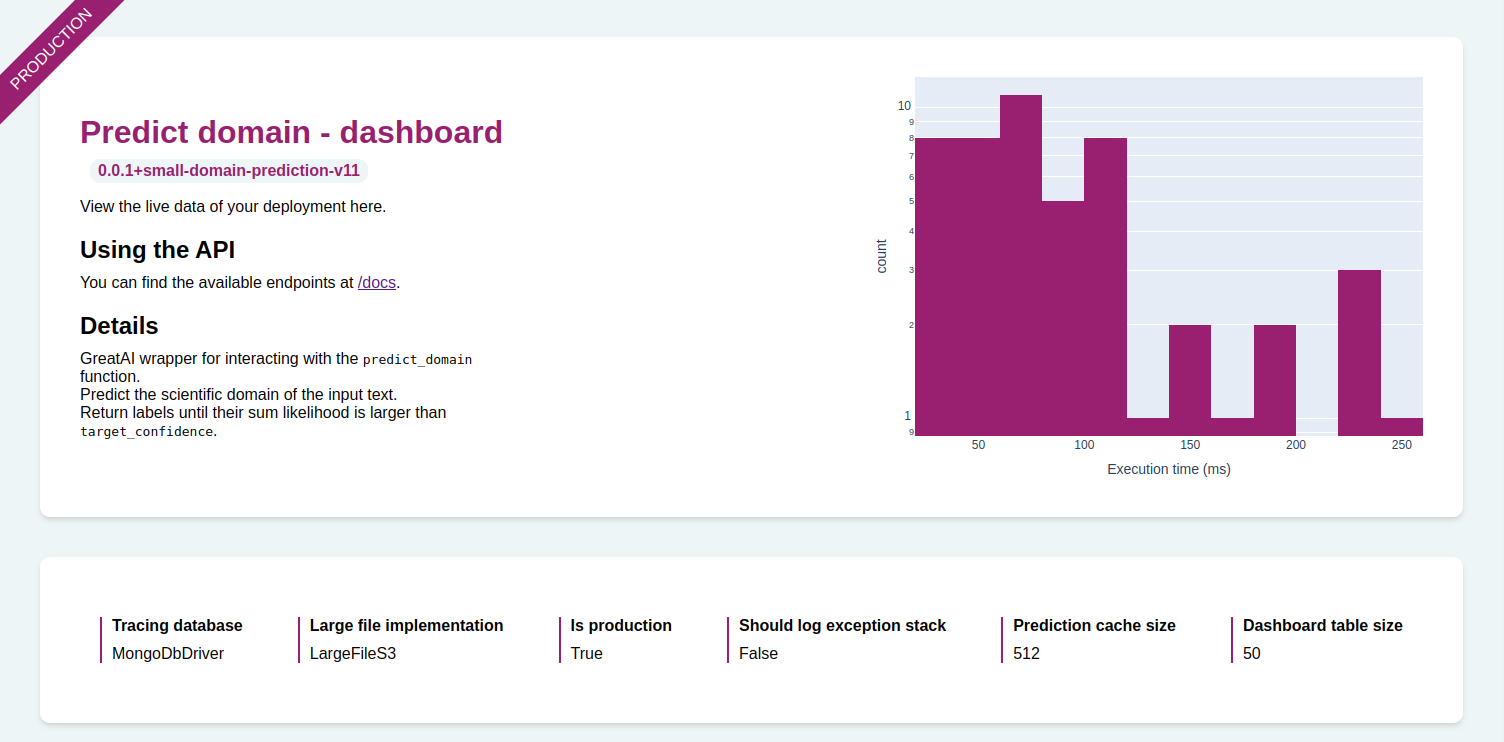
\includegraphics[width=1\linewidth]{figures/greatai-header.png}
    \captionsetup{width=.9\linewidth}
    \caption{The header of the automatically generated dashboard of the service from Section \ref{section:simple-case}. A generated documentation is shown on the left, while the histogram of response times is rendered on the right. The current configuration is prominently displayed on the bottom.}
    \label{fig:greatai-header}
\end{figure}

\begin{figure}
    \centering
    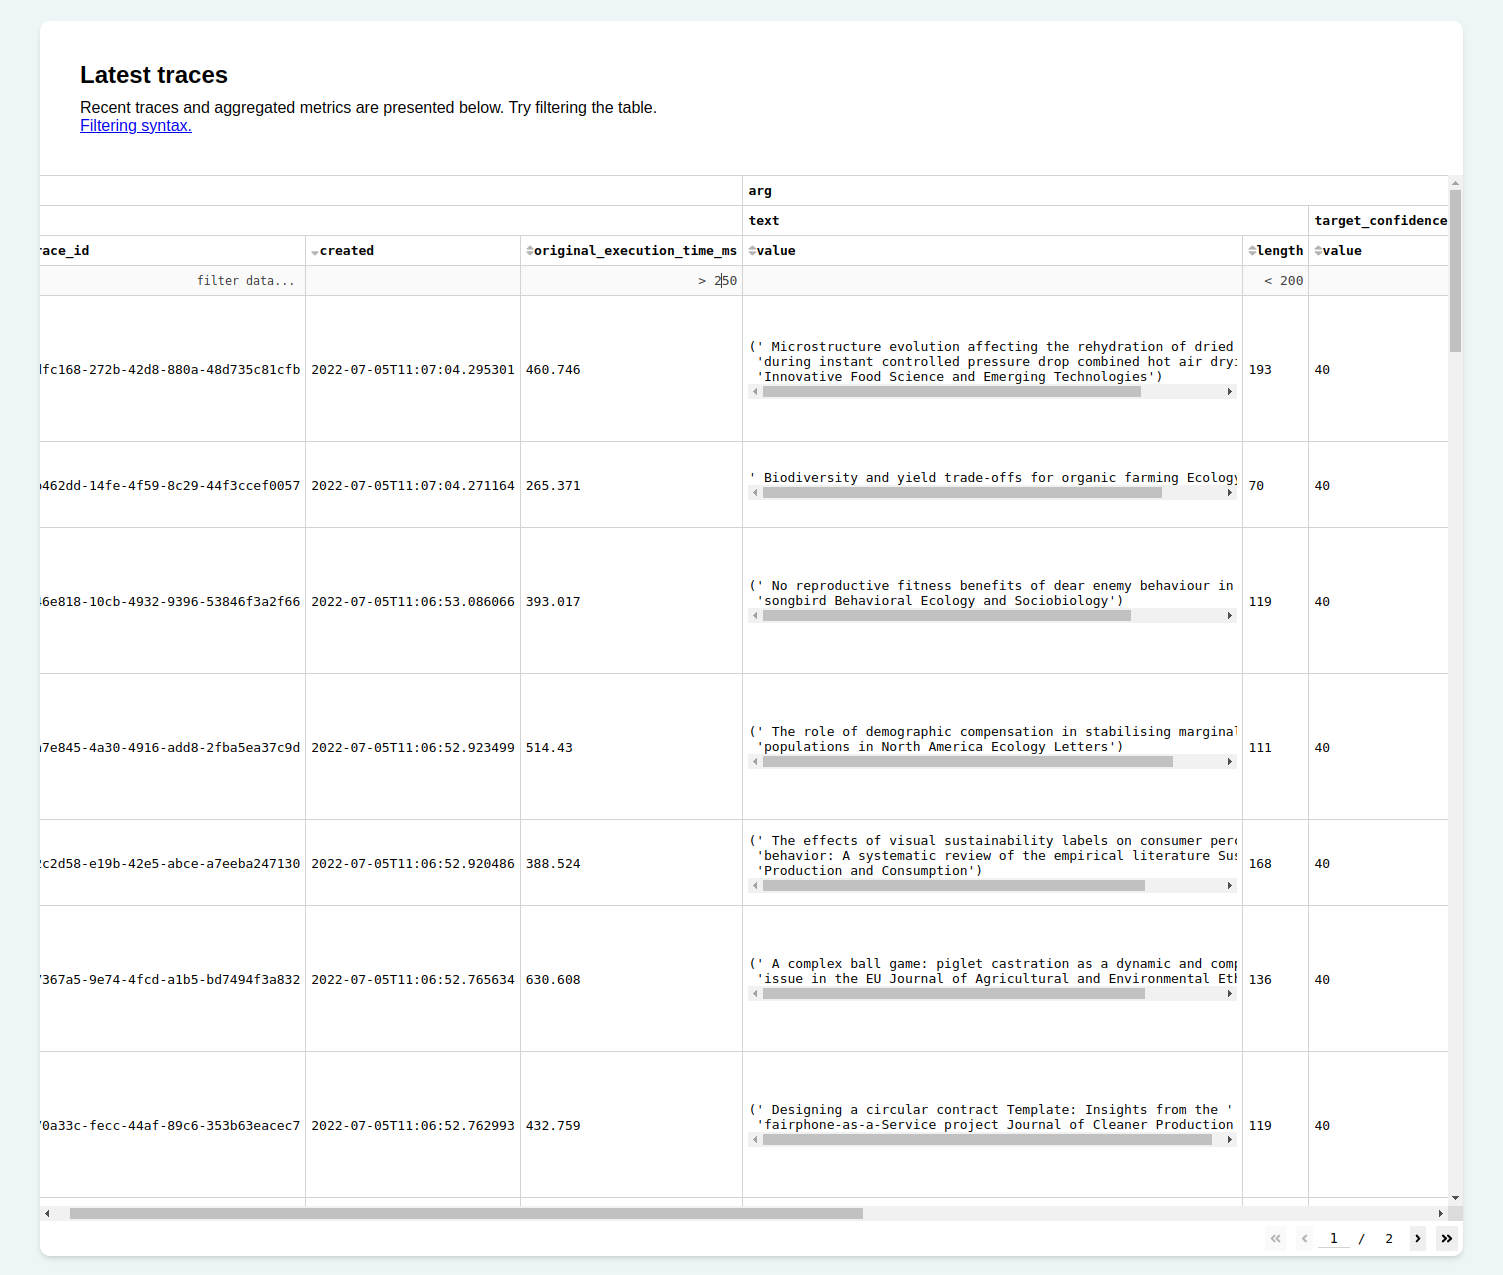
\includegraphics[width=1\textwidth]{figures/greatai-table.png}
    \captionsetup{width=.9\linewidth}
    \caption{A dynamically updating, tabular view of traces matching a user-defined filter. Useful for exploring historical predictions or debugging the cause of exceptions (which are also searchable). The filters set in the table affect the other diagrams of the dashboard.}
    \label{fig:greatai-table}
\end{figure}

\begin{figure}
    \centering
    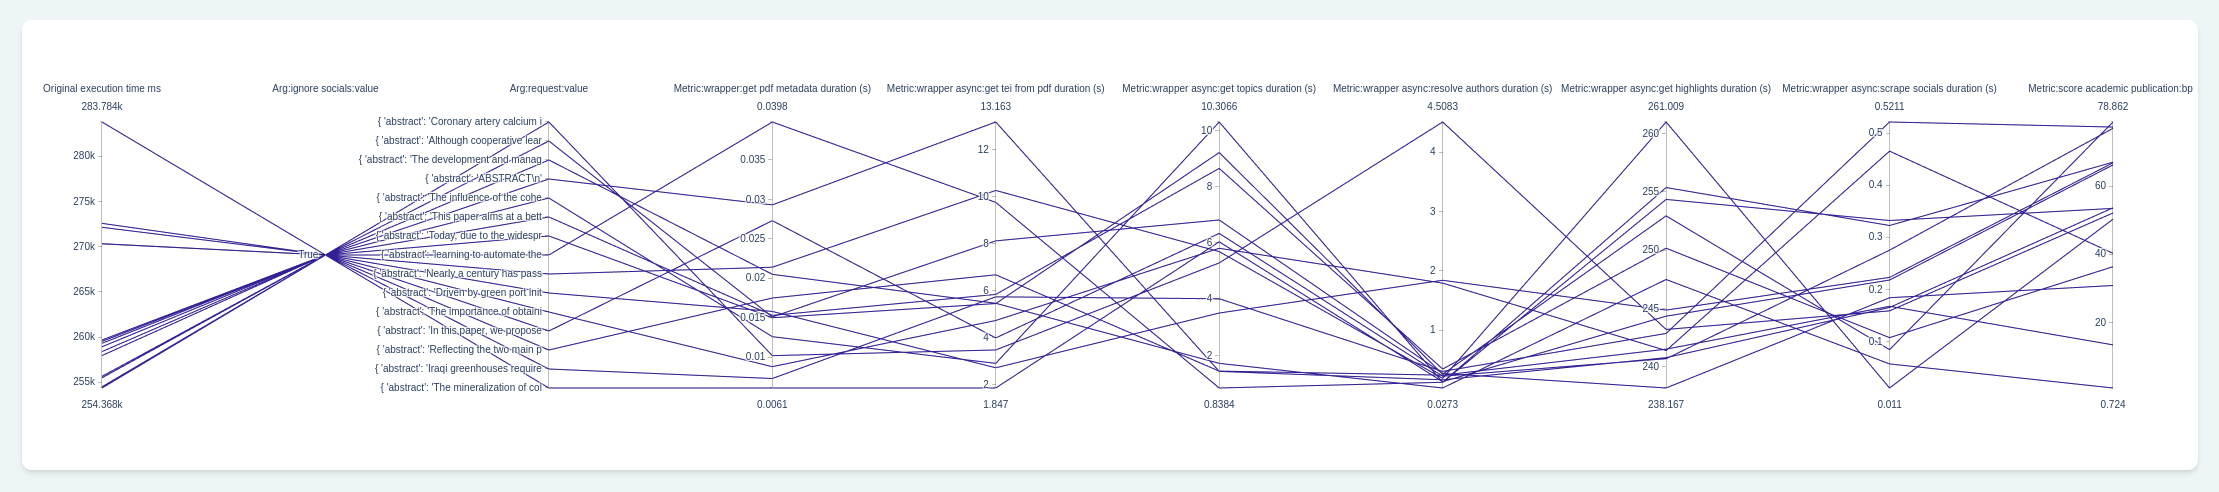
\includegraphics[width=1\textwidth]{figures/greatai-parallel.png}
    \captionsetup{width=.9\linewidth}
    \caption{A parallel coordinates view of the traces displayed in the table above. Adding new axes is as easy as calling \texttt{log\_metric} inside the inference function.}
    \label{fig:greatai-parallel}
\end{figure}
